\section{Spheres \& Shells}
\label{sect:Spheres_Shells}

\subsection{Sphere}
\label{sect:sphere} ~\\

\begin{figure}[htb]
\begin{center}
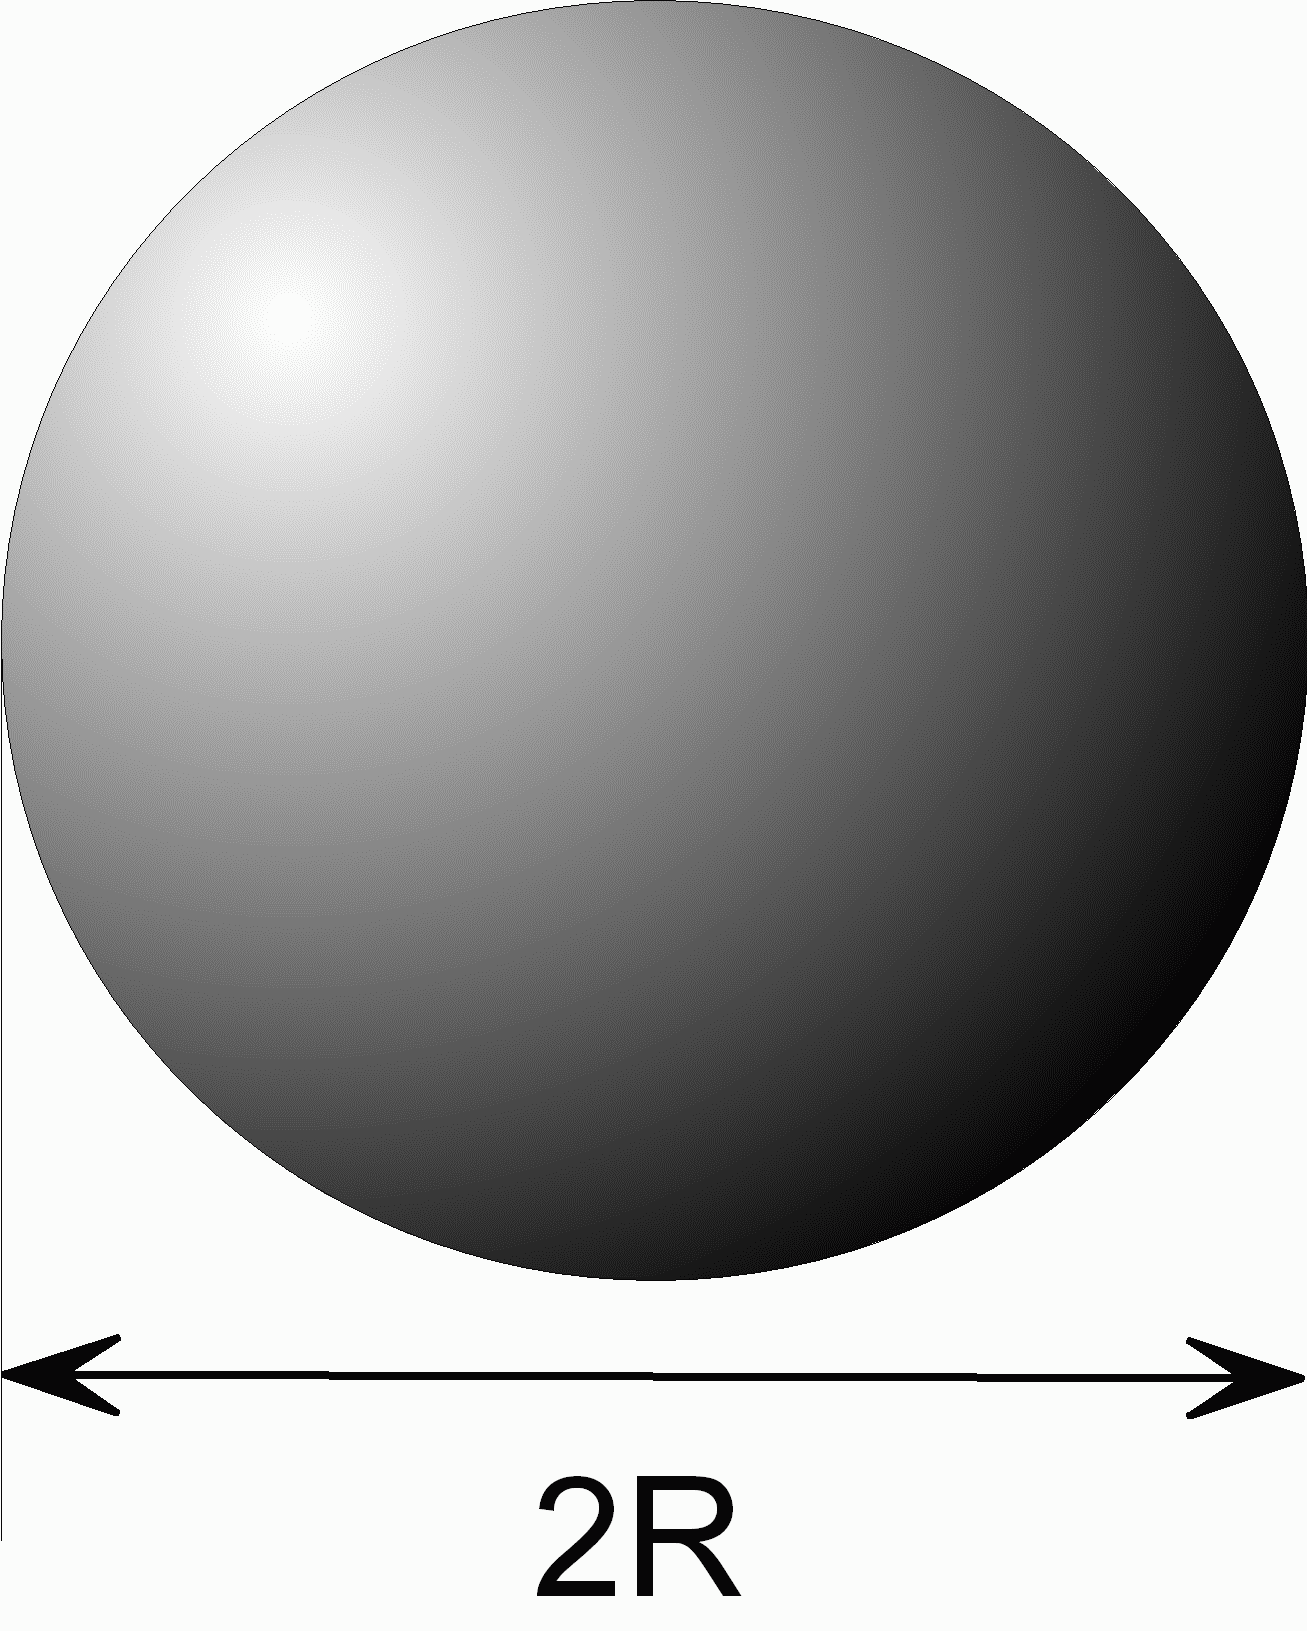
\includegraphics[width=0.2875\textwidth]{../images/form_factor/spheres/sphere.png}
\end{center}
\caption{Sphere with diameter $2R$} \label{fig:Sketch_sphere}
\end{figure}
The scattering intensity and scattering amplitude of a homogeneous sphere with a small relative refraction index is given by \cite{Rayleigh1914}
\begin{subequations}
\begin{align}
I_\text{Sphere}(Q,R) = K^2(Q,R,\Delta\eta) \label{eq:I_sphere}
\end{align}
with
\begin{align}
 K(Q,R,\Delta\eta) = \frac{4}{3}\pi R^3 \Delta\eta \, 3 \frac{\sin QR - QR \cos QR}{(QR)^3}
\end{align}
The forward scattering for $Q=0$ is given by
$$
\lim_{Q=0}I_\text{Sphere}(Q,R) =\left( \frac{4}{3}\pi R^3 \Delta\eta \right)^2
$$
\end{subequations}

\vspace{5mm}
\noindent \underline{Input Parameters for model \texttt{Sphere}:}
\begin{description}
\item[\texttt{R}] radius of sphere $R$
\item[- - -] not used
\item[- - -] not used
\item[\texttt{eta}] scattering length density difference between particle and matrix $\Delta\eta$
\end{description}

\noindent\underline{Note:}
\begin{itemize}
\item The parameters \texttt{param.p[1]} and \texttt{param.p[2]} are not used.
\end{itemize}

\begin{figure}[htb]
\begin{center}
\includegraphics[width=0.768\textwidth]{../images/form_factor/spheres/sphere_P.png}
\end{center}
\caption{Scattering intensity of spheres with radii $R=10$nm and $R=20$nm.
The scattering length density contrast is set to 1.} \label{fig:I_sphere}
\end{figure}

%%%%%%%%%%%%%%%%%%%%%%%%%%%%%%%%%%%%%%%%%%%%%%%%%%%%%%%%%%
\clearpage

\subsection{Spherical Shell i}
\label{sect:spherical_shell_i} ~\\

\begin{figure}[htb]
\begin{center}
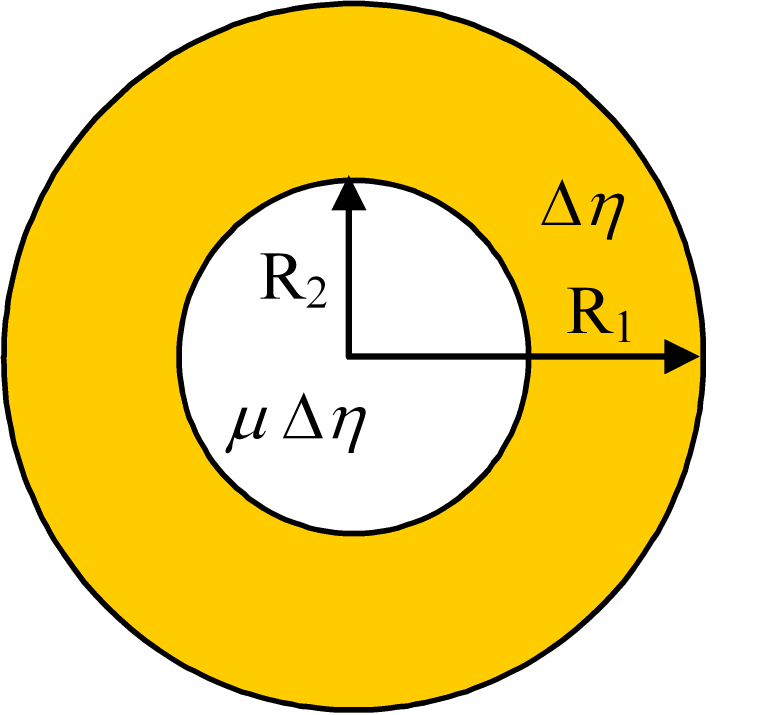
\includegraphics[width=0.38\textwidth]{../images/form_factor/spheres/shell1.png}
\end{center}
\caption{Spherical Shell i} \label{fig:shell1}
\end{figure}

This implementation of a spherical shell is parametrised with an inner radius $ R_2$ and outer
radius $R_1$. The scattering contrast relative to the matrix of the core is $\mu \Delta \eta$
and the one of the shell $\Delta\eta$.

\begin{align}
I_\text{Shell1}(Q,R_1,R_2,\Delta\eta,\mu)=
\left[K(Q,R_1,\Delta\eta)-K(Q,R_2,\Delta\eta(1-\mu))\right]^2
\end{align}
with
\begin{align}
 K(Q,R,\Delta\eta) = \frac{4}{3}\pi R^3 \Delta\eta \, 3 \frac{\sin QR - QR \cos QR}{(QR)^3}
\end{align}
The forward scattering for $Q=0$ is given by
$$
\lim_{Q=0}I_\text{Shell1}(Q,R_1,R_2,\Delta\eta,\mu) =
\left(\frac{4}{3}\pi \Delta\eta \left[ R_1^3 -
R_2^3(1-\mu)\right]\right)^2
$$

\vspace{5mm}
\noindent  \underline{Input Parameters for model \texttt{Spherical Shell i}:}
\begin{description}
\item[\texttt{R1}] overall radius of spherical shell $R_1$
\item[\texttt{R2}] radius of core $R_2$
\item[\texttt{eta}] scattering length density difference between shell and matrix $\Delta\eta$
\item[\texttt{mu}] scattering length density difference between core and matrix relative to the shell contrast $\mu$
\end{description}

\noindent\underline{Note:}
\begin{itemize}
\item[~] None
\end{itemize}

\begin{figure}[htb]
\begin{center}
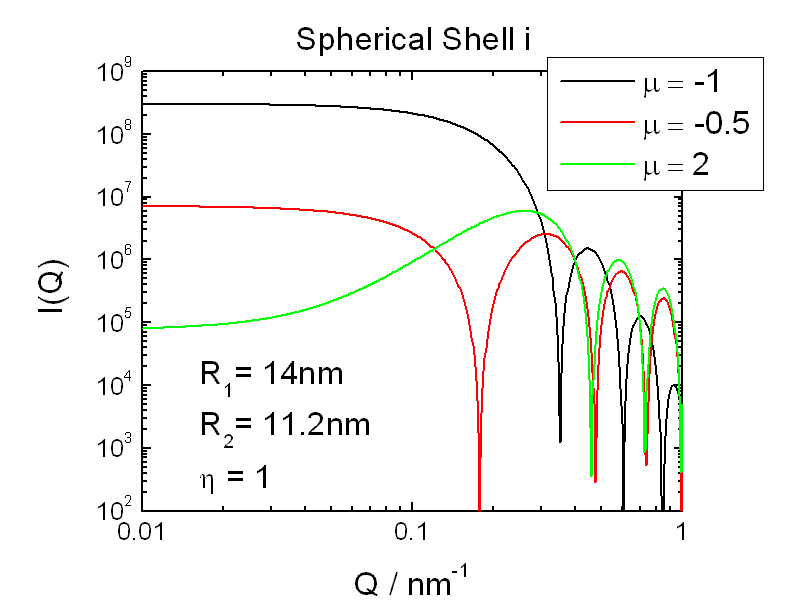
\includegraphics[width=0.768\textwidth]{../images/form_factor/spheres/shell_i_P.png}
\end{center}
\caption{Scattering intensity of spherical shell with outer radius of $R_1=14$nm
and inner radius of $R_2=11.2$nm. The scattering length density contrast the shell is set to 1
and the one of the core to -1, -0.5, and 2.} \label{fig:I_shell_i}
\end{figure}


%%%%%%%%%%%%%%%%%%%%%%%%%%%%%%%%%%%%%%%%%%%%%%%%%%%%%%%%%%%
\clearpage
\subsection{Spherical Shell ii}
\label{sect:spherical_shell_ii} ~\\

\begin{figure}[htb]
\begin{center}
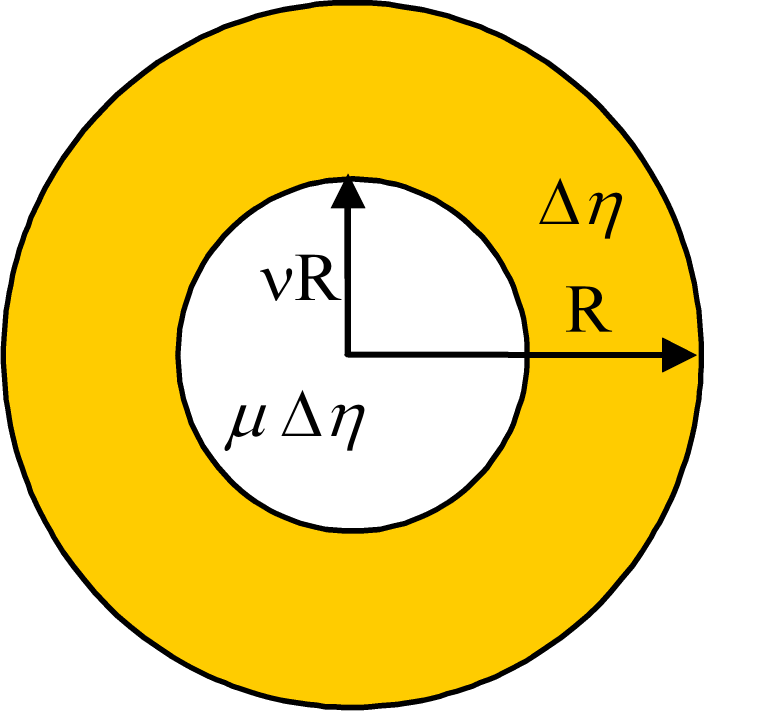
\includegraphics[width=0.38\textwidth]{../images/form_factor/spheres/shell2.png}
\end{center}
\caption{\texttt{Spherical Shell ii}} \label{fig:shell2}
\end{figure}
This implementation of a spherical shell is parametrised with an outer radius $R$ and an inner
radius $\nu R$. The scattering contrast relative to the matrix of the core is $ \mu \Delta \eta$
and the one of the shell $\Delta\eta$.
\begin{align}
I_\text{Shell2}(Q,R,\nu,\Delta\eta,\mu)=
\left(K(Q,R,\Delta\eta)-K(Q,\nu R,\Delta\eta(1-\mu))\right)^2
\end{align}
with
\begin{align}
 K(Q,R,\Delta\eta) = \frac{4}{3}\pi R^3 \Delta\eta \, 3 \frac{\sin QR - QR \cos QR}{(QR)^3}
\end{align}
The forward scattering for $Q=0$ is given by
$$
\DS \lim_{Q=0}I_\text{Shell2}(Q,R,R,\Delta\eta,\mu) =
\left(\frac{4}{3}\pi \Delta\eta \left[ R^3 - \nu^3
R^3(1-\mu)\right]\right)^2
$$

\vspace{5mm}
\noindent \underline{Input Parameters for model \texttt{Spherical Shell ii}:}
\begin{description}
\item[\texttt{R}] overall radius of spherical shell $R$
\item[\texttt{nu}] the radius of the core is only the fraction $\nu$ of the overall radius  $R$
\item[\texttt{eta}] scattering length density difference between shell and matrix $\Delta\eta$
\item[\texttt{mu}] scattering length density difference between core and matrix relative to the shell contrast $\mu$
\end{description}

\noindent\underline{Note:}
\begin{itemize}
\item[~] None
\end{itemize}

\begin{figure}[htb]
\begin{center}
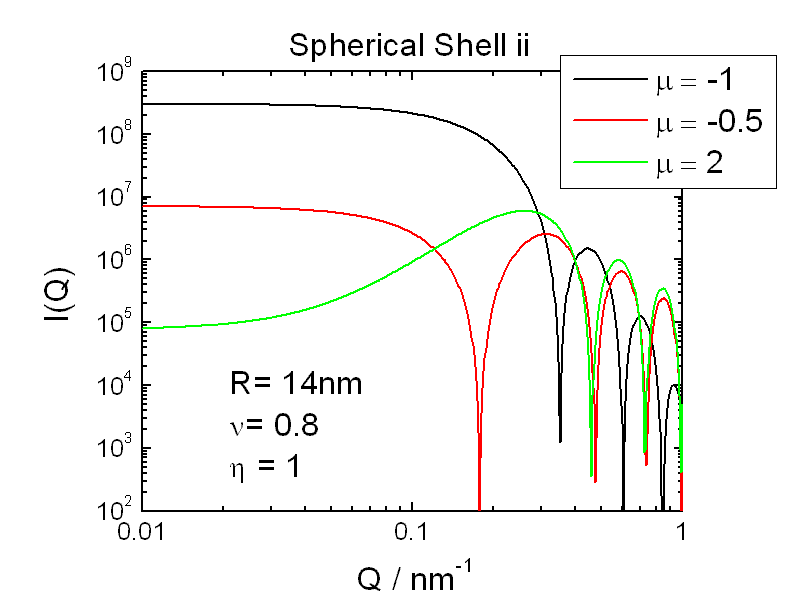
\includegraphics[width=0.768\textwidth]{../images/form_factor/spheres/shell_ii_P.png}
\end{center}
\caption{Scattering intensity of spherical shell with outer radius of $R=14$nm
and inner radius of $\nu R=11.2$nm. The scattering length density contrast the shell is set to 1
and the one of the core to -1, -0.5, and 2.} \label{fig:I_shell_ii}
\end{figure}

%%%%%%%%%%%%%%%%%%%%%%%%%%%%%%%%%%%%%%%%%%%%%%%%%%%%%%%%%%%%%%%
\clearpage
\subsection{Spherical Shell iii}
\label{sect:spherical_shell_iii} ~\\

\begin{figure}[htb]
\begin{center}
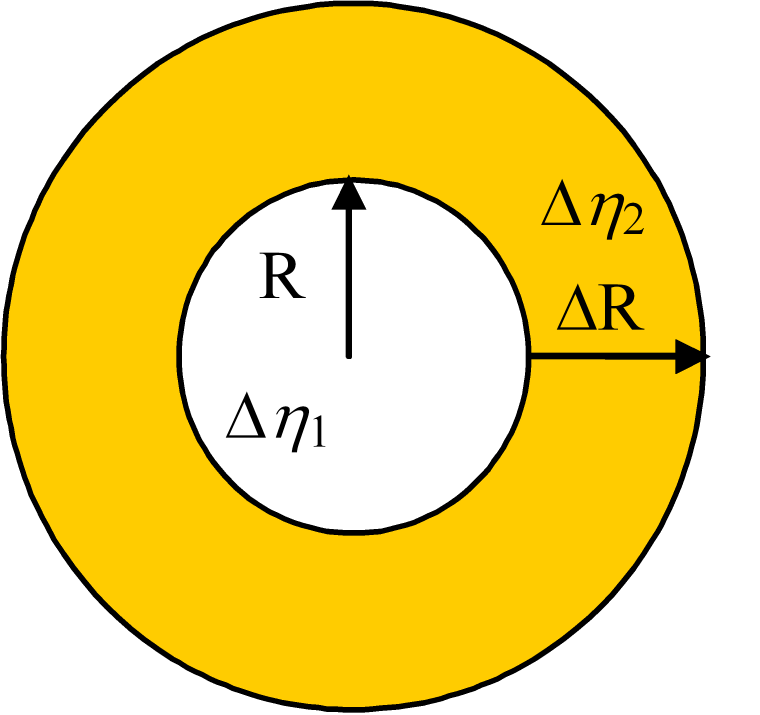
\includegraphics[width=0.38\textwidth]{../images/form_factor/spheres/shell3.png}
\end{center}
\caption{Spherical Shell iii} \label{fig:shell3}
\end{figure}
This implementation of a spherical shell is parametrised with an inner radius $R$ and a shell
thickness $\Delta R$. The scattering contrast relative to the matrix of the core is $ \Delta \eta_1$
and the one of the shell $\Delta\eta_2$.
\begin{align}
I_\text{Shell3}(Q,R,\Delta R,\Delta\eta_1,\Delta\eta_2)=
\left[K(Q,R+\Delta
R,\Delta\eta_2)-K(Q,R,\Delta\eta_2-\Delta\eta_1)\right]^2
\end{align}
with
\begin{align}
 K(Q,R,\Delta\eta) = \frac{4}{3}\pi R^3 \Delta\eta \, 3 \frac{\sin QR - QR \cos QR}{(QR)^3}
\end{align}
The forward scattering for $Q=0$ is given by
$$
\DS \lim_{Q=0}I_\text{Shell3}(Q,R,\Delta R,\Delta\eta_1,\Delta\eta_2)
= \left(\frac{4}{3}\pi \left[(R+\Delta R)^3\Delta\eta_2
                            - R^3(\Delta\eta_2-\Delta\eta_1)\right]\right)^2
$$

\vspace{5mm}
\noindent  \underline{Input Parameters for model \texttt{Spherical Shell iii}:}
\begin{description}
\item[\texttt{R}] radius of core $R$
\item[\texttt{dR}] thickness of the shell $\Delta R$
\item[\texttt{eta1}] scattering length density difference between core and matrix $\Delta\eta_1$
\item[\texttt{eta2}] scattering length density difference between shell and matrix $\Delta\eta_2$
\end{description}

\noindent\underline{Note:}
\begin{itemize}
\item[~] None
\end{itemize}


\begin{figure}[htb]
\begin{center}
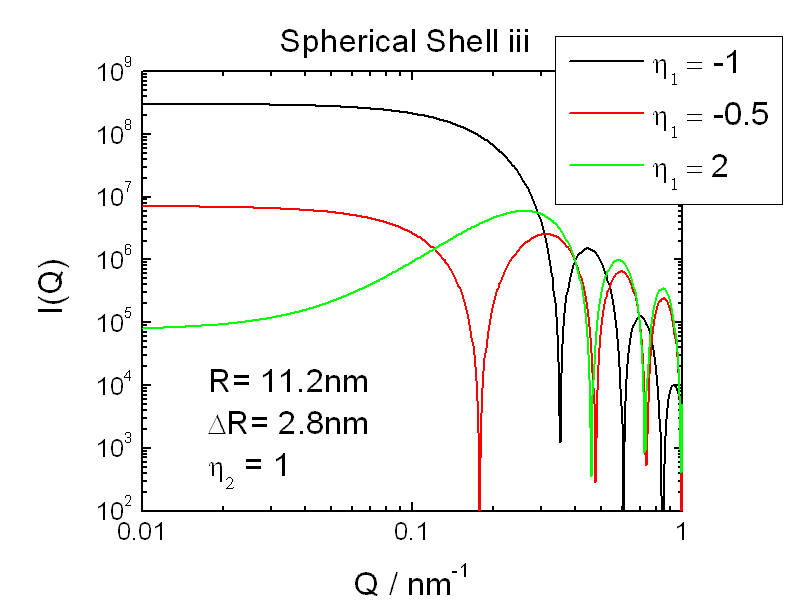
\includegraphics[width=0.768\textwidth]{../images/form_factor/spheres/shell_iii_P.png}
\end{center}
\caption{Scattering intensity of spherical shell with core radius of $R=11.2$nm
and shell thickness of $\Delta R=2.8$nm. The scattering length density contrast the shell is set to 1
and the one of the core to -1, -0.5, and 2.} \label{fig:I_shell_iii}
\end{figure}
\clearpage


%%%%%%%%%%%%%%%%%%%%%%%%%%%%%%%%%%%%%%%%%%%%%%%%%%%%%%%%%%%%%%%%%%%%%%%%%%

\clearpage
\subsection{Bilayered Vesicle}
\label{sect:BilayeredVesicle} ~\\

\begin{figure}[htb]
\begin{center}
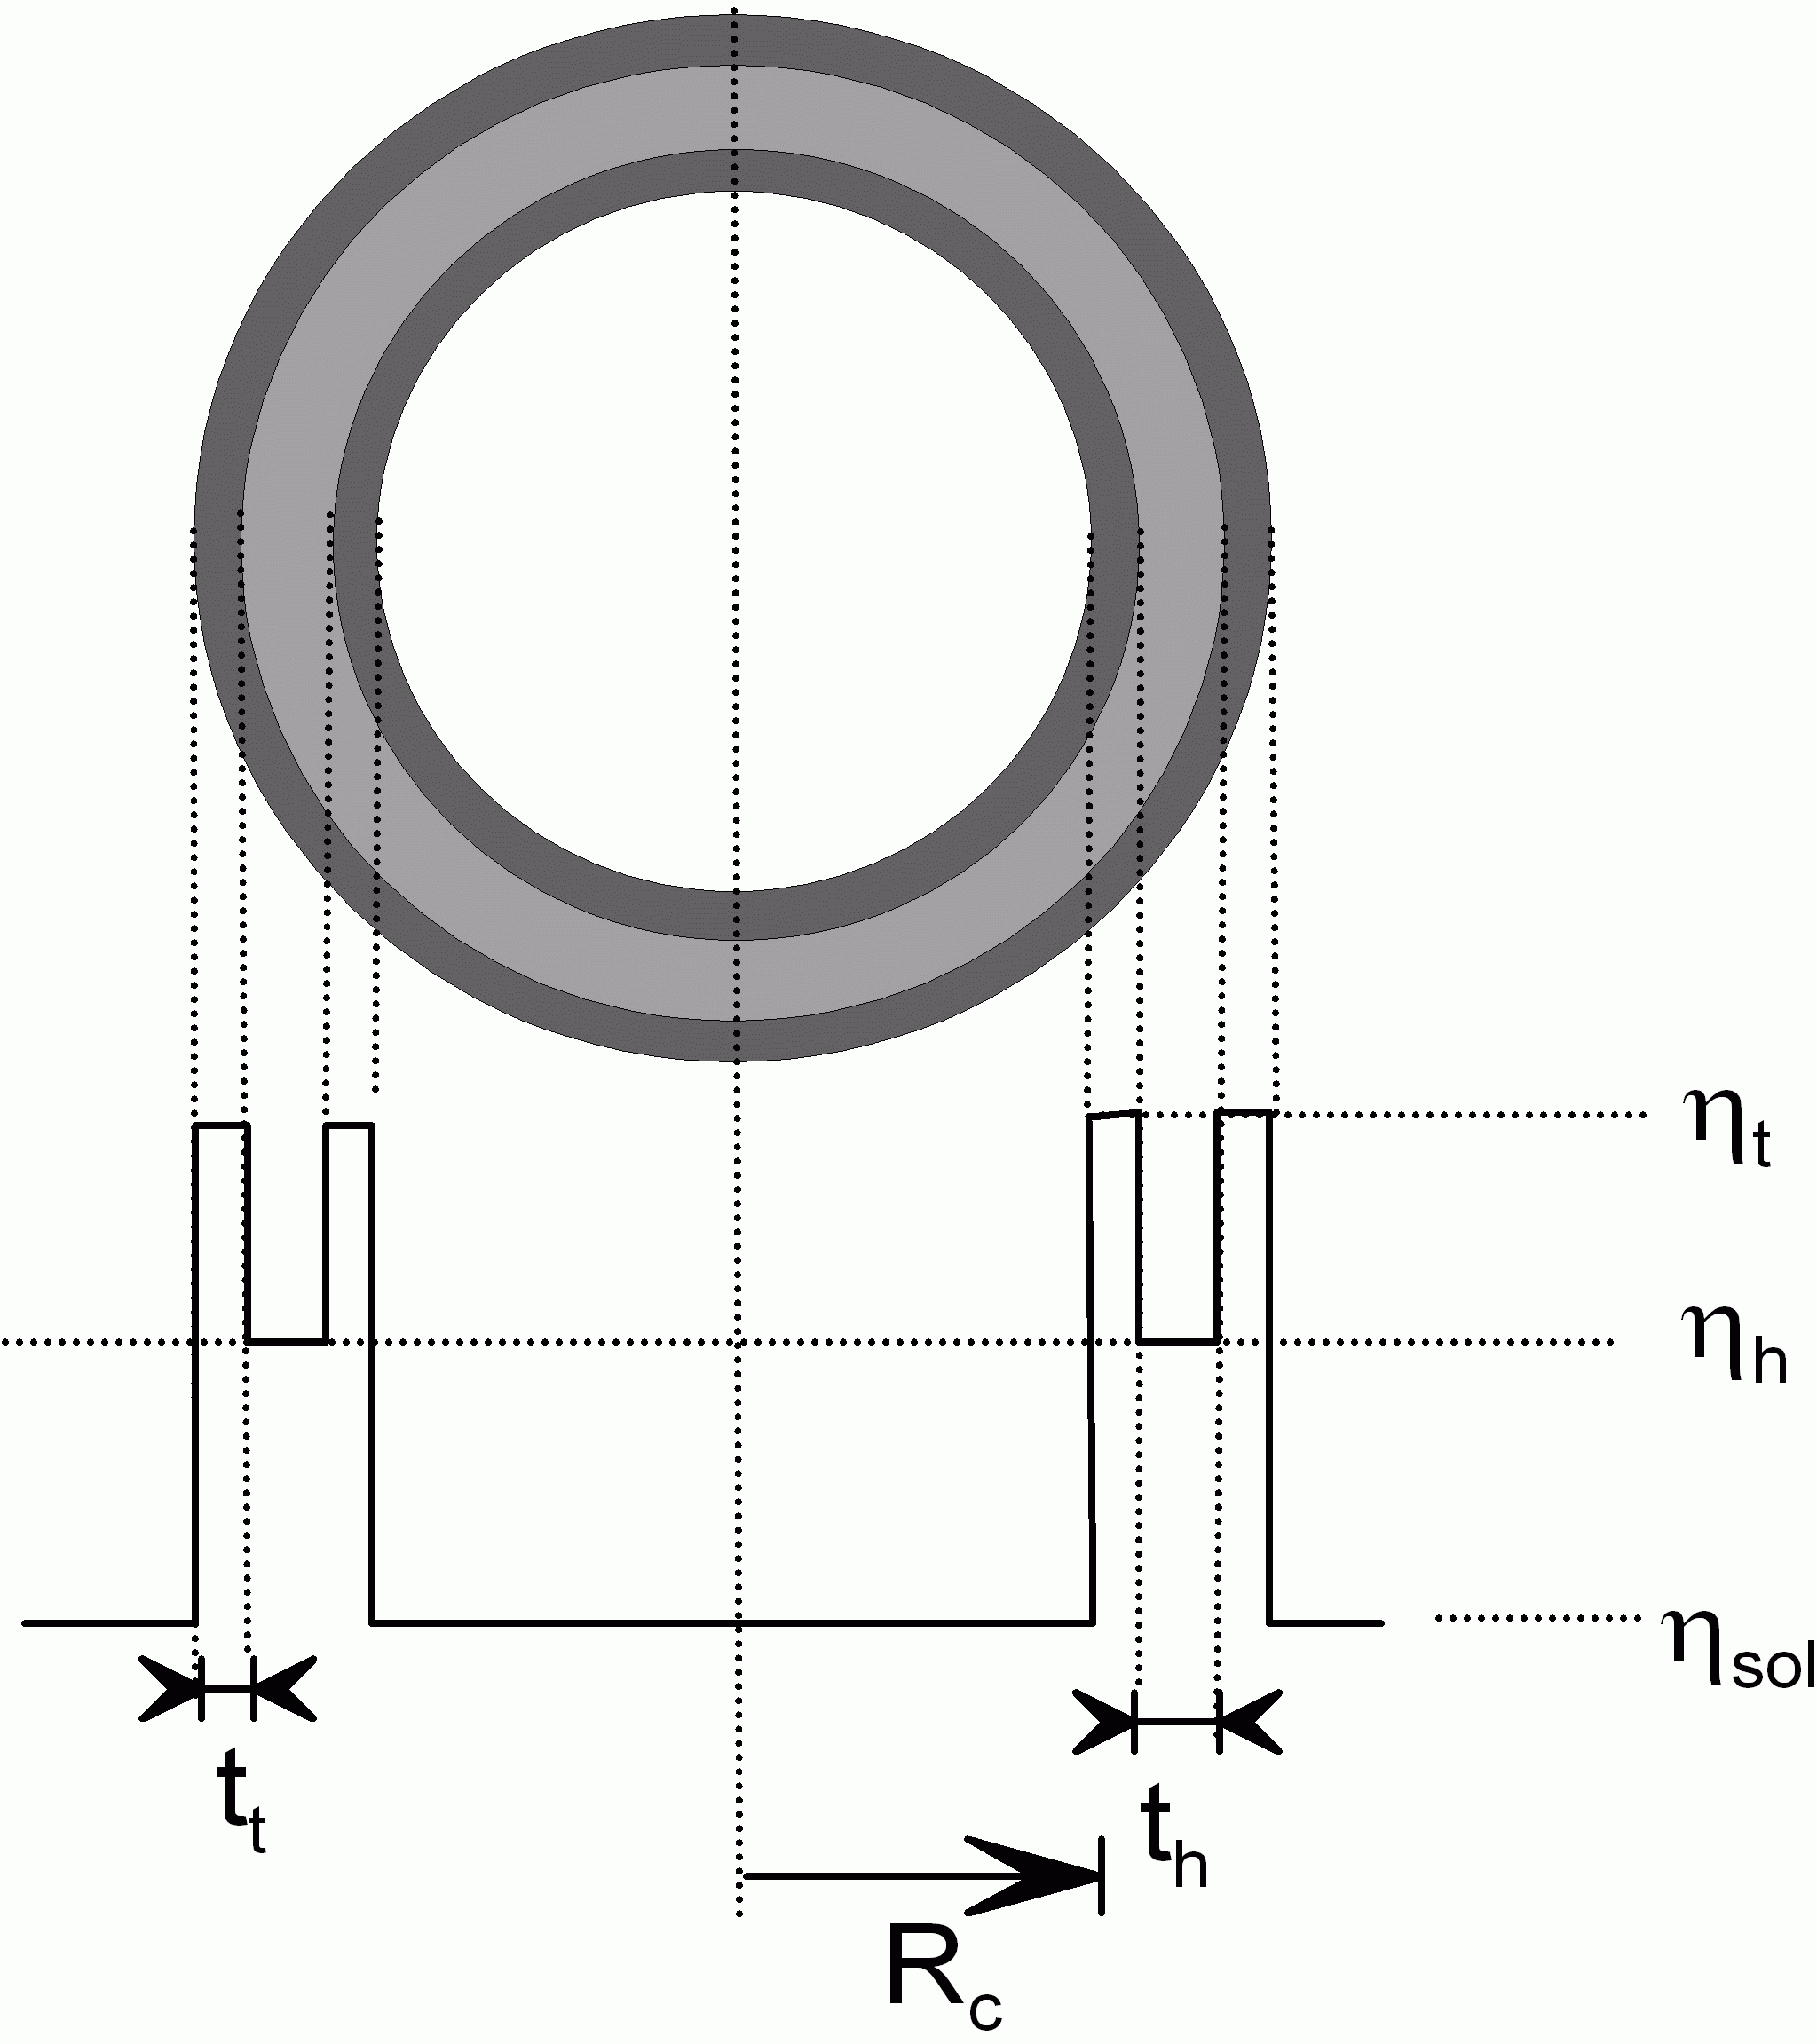
\includegraphics[width=0.5441\textwidth]{../images/form_factor/spheres/BiLayeredVesicle.png}
\end{center}
\caption{BiLayeredVesicle} \label{fig:BiLayeredVesicle}
\end{figure}
\begin{align}
I_\text{BLV}(Q) = \bigg( & + K(Q,R_c,\eta_{sol}-\eta_{t})+ K(Q,R_c+t_{t},\eta_{t}-\eta_{h}) \\
&+ K(Q,R_c+t_{t}+t_{h},\eta_{h}-\eta_{t}) +
K(Q,R_c+2t_{t}+t_{h},\eta_{t}-\eta_{sol}) \bigg)^2 \nonumber
\end{align}
with
\begin{align}
 K(Q,R,\Delta\eta) = \frac{4}{3}\pi R^3 \Delta\eta \, 3 \frac{\sin QR - QR \cos QR}{(QR)^3}
\end{align}

\vspace{5mm}
\hspace{1pt}\\
\underline{Input Parameters for model \texttt{BilayeredVesicle}:}\\
\begin{description}
\item[\texttt{R\_c}] radius of core $R_c$ which consists of solvent
\item[\texttt{t\_h}] thickness of outer part of bilayer (in contact with solvent, head group) $t_\text{h}$
\item[\texttt{t\_t}] thickness of inner part of bilayer (tail group) $t_\text{t}$
\item[\texttt{eta\_sol}] scattering length density of solvent $\eta_\text{sol}$
\item[\texttt{eta\_h}] scattering length density of outer part of bilayer $\eta_\text{h}$
\item[\texttt{eta\_t}] scattering length density of inner part of bilayer $\eta_\text{t}$
\end{description}

\noindent\underline{Note:}
\begin{itemize}
\item[~] None
\end{itemize}

\begin{figure}[htb]
\begin{center}
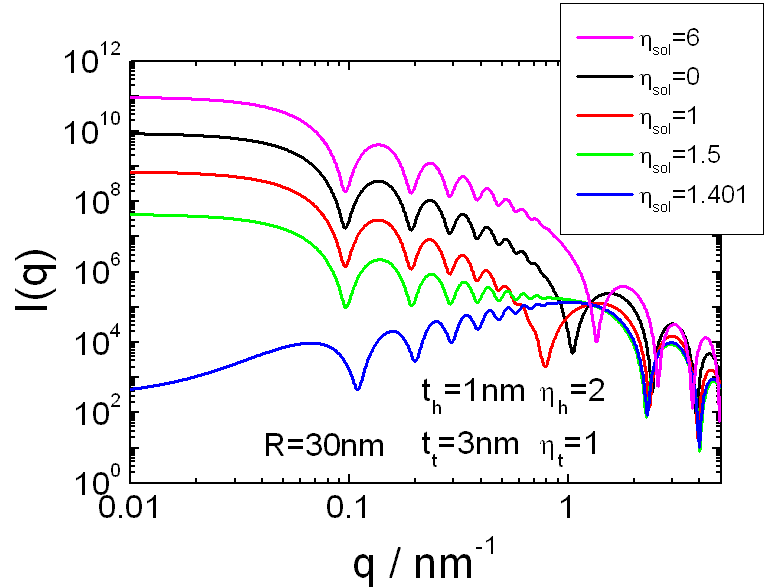
\includegraphics[width=0.768\textwidth]{../images/form_factor/spheres/bilayered_vesicle.png}
\end{center}
\caption{Scattering intensity of a bilayered vesicle. The scattering intensity has been calculated
with a lognormal $[\mathrm{LogNorm}(N\!=\!1,\sigma\!=\!0.05,p\!=\!1,R\!=\!30)]$ size distribution for the vesicle radius $R_c$.}
\label{fig:I_BiLayeredVesicle}
\end{figure}

%%%%%%%%%%%%%%%%%%%%%%%%%%%%%%%%%%%%%%%%%%%%%%%%%%%%%%%%%%%%%%%%%%

\clearpage
\subsection{Multi Lamellar Vesicle}
\label{sect:MultiLamellarVesicle} ~\\

\begin{figure}[htb]
\begin{center}
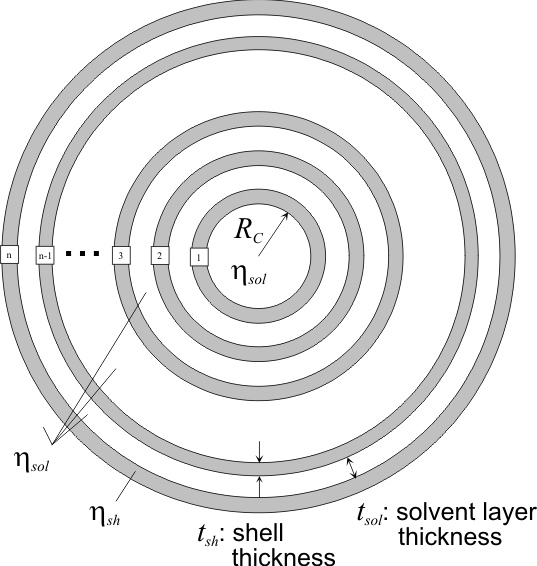
\includegraphics[width=0.537\textwidth]{../images/form_factor/spheres/multilamellar_vesicle.png}
\end{center}
\caption{MultiLamellarVesicle} \label{fig:MultiLamellarVesicle}
\end{figure}
\begin{align}
I_\text{MLV}(Q) = \Bigg( \sum_{i=0}^{n-1} \bigg[ & K(Q,R_c+it_{sh}+it_{sol},\eta_{sol}-\eta_{sh}) \nonumber \\
+ &K(Q,R_c+(i+1)t_{sh}+it_{sol},\eta_{sh}-\eta_{sol}) \bigg]
\Bigg)^2
\end{align}
with
\begin{align}
 K(Q,R,\Delta\eta) = \frac{4}{3}\pi R^3 \Delta\eta \, 3 \frac{\sin QR - QR \cos QR}{(QR)^3}
\end{align}


\noindent\underline{Input Parameters for model \texttt{MultiLamellarVesicle}:}
\begin{description}
\item[\texttt{R\_c}] radius of core $R_c$ which consists of solvent
\item[\texttt{t\_sh}] surfactant layer thickness $t_\text{sh}$
\item[\texttt{t\_sol}] thickness of solvent layer $t_\text{sol}$
\item[\texttt{eta\_sh}] scattering length density of surfactant layer $\eta_\text{sh}$
\item[\texttt{eta\_sol}] scattering length density of solvent $\eta_\text{sol}$
\item[\texttt{n}] total number of surfactant layers $n$
\end{description}

\noindent\underline{Note:}
\begin{itemize}
\item[~] None
\end{itemize}


\begin{figure}[htb]
\begin{center}
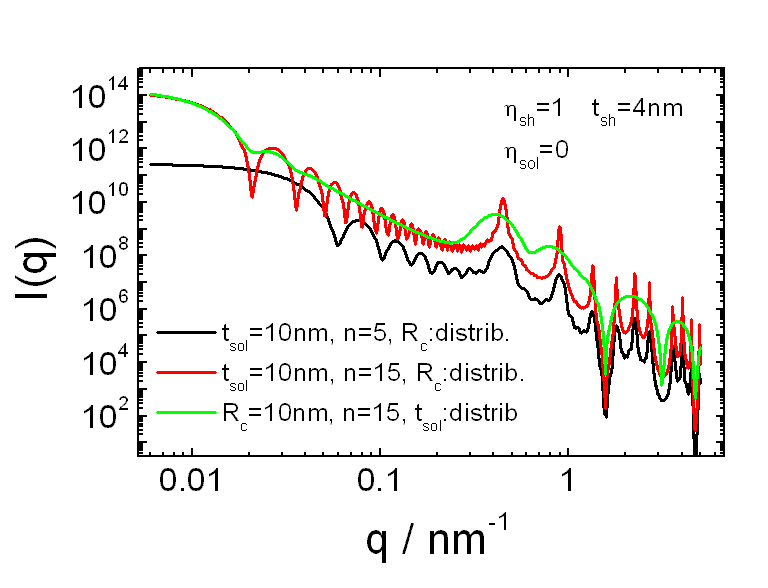
\includegraphics[width=0.768\textwidth]{../images/form_factor/spheres/multilamellar_vesicle_Iq.png}
\end{center}
\caption{Scattering intensity of a multilamellar vesicle. The scattering intensities has been calculated
for a\&b) a distribution of the core radius $R_c$ by
$\int\mathrm{LogNorm}(R_c;N\!=\!1,\sigma\!=\!0.3,p\!=\!1,R\!=\!10) I(q,R_c)\, \mathrm{d}R_c$
and c) for a distribution of the distances between the lamellars
$\int\mathrm{LogNorm}(t_\text{sol};N\!=\!1,\sigma\!=\!0.3,p\!=\!1,R\!=\!10) I(q,t_\text{sol})\, \mathrm{d}t_\text{sol}$.}
\label{fig:I_MLV}
\end{figure}

%%%%%%%%%%%%%%%%%%%%%%%%%%%%%%%%%%%%%%%%%%%%%%%%%%%%%%%%%%%%%%%%%%

\clearpage
\subsection{RNDMultiLamellarVesicle}
\label{sect:RNDMultiLamellarVesicle} ~\\

\begin{figure}[htb]
\begin{center}
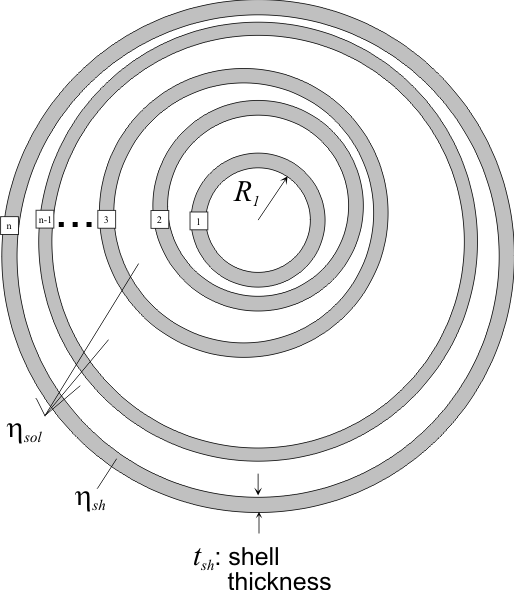
\includegraphics[width=0.537\textwidth]{../images/form_factor/spheres/random_multilamellar_vesicle.png}
\end{center}
\caption{randomMultiLamellarVesicle}
\label{fig:randomMultiLamellarVesicle}
\end{figure}
\begin{align}
I_\text{RndMLV}(Q) &= \Delta\eta ^2 \sum_{i=1}^{N} F_i^2(q,R_i,t_{sh,i}) \nonumber \\
&+ \Delta\eta ^2 \sum_{i<j}^{N} 2 F_i(q,R_i,t_{sh,i}) F_j(q,R_j,t_{sh,j}) \frac{\sin qr_{ij}}{qr_{ij}}
\end{align}
with
\begin{subequations}
\begin{align}
r_{ij} & = \abs{\mathbf{R}_i-\mathbf{R}_j} \\
F_i(q,R_i,t_{sol,i}) &= K(q,R_i+t_{sol,i},\Delta\eta)-K(q,R_i,\Delta\eta)\\
K(q,R,\Delta\eta) &= \frac{4}{3}\pi R^3 \Delta\eta \, 3 \frac{\sin qR - qR \cos qR}{(qR)^3}
\end{align}
\end{subequations}

\begin{subequations}
\begin{align}
R_1 &= \textrm{ran}_{lognormal}\left(\log(R_c),\sigma_{R_c}\right) \\
\Delta R_{i} &= \textrm{ran}_{gaussian}\left(\sigma_{t_{sol}}\right) \\
R_i &= R_{i-1}+t_{sh,i-1}+\Delta R_{i}\\
\mathbf{R}_i &= R_i \; \textbf{ran}_{dir,3D}
                       \text{ran}_{uniform} \; \Delta t_{sol}
\end{align}
\end{subequations}


\hspace{1mm}\\
\underline{Input Parameters for model
\texttt{RNDMultiLamellarVesicle}:}
\begin{description}
\item[\texttt{t\_sh}] average surfactant layer thickness $t_\text{sh}$
\item[\texttt{s\_sh}] Gaussian thickness distribution of surfactant layer with a width of $\sigma_\text{sh}$
\item[\texttt{R\_c}] average radius of core $R_c$ which consists of solvent
\item[\texttt{s\_c}] lognormal size distribution of core radius $R_c$ with a width of $\sigma_c$
\item[\texttt{n}] average number of surfactant layers $n$
\item[\texttt{s\_n}] lognormal distribution of the number of surfactant layers with a width of $\sigma_n$
\item[\texttt{t\_sol}] average thickness of solvent layer $t_\text{sol}$
\item[\texttt{s\_sol}] lognormal thickness distribution of solvent layer with a width of $\sigma_\text{sol}$
\item[\texttt{Deta\_sh}] scattering length density contrast $\Delta\eta$ between surfactant layer and solvent
\end{description}

\noindent\underline{Note:}
\begin{itemize}
\item[~] The number of Monte Carlo iterations can be set via the menu \texttt{[Options|Customize...]}
\end{itemize}

\begin{figure}[htb]
\begin{center}
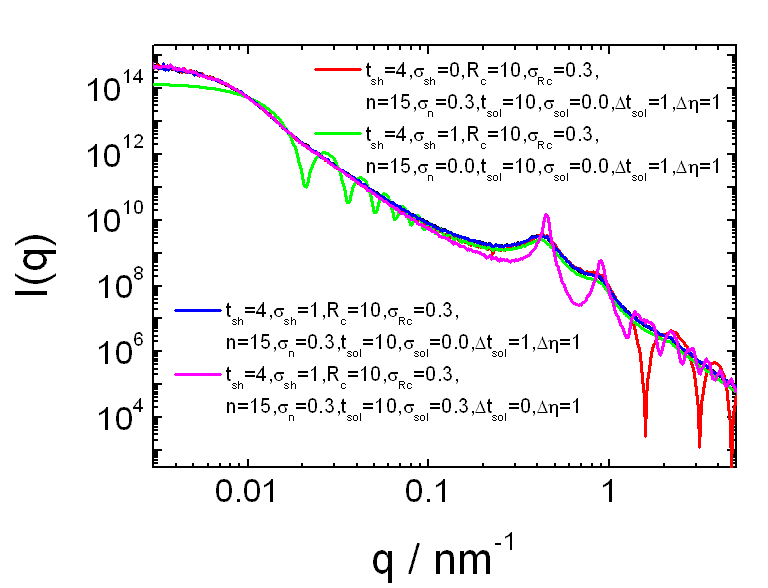
\includegraphics[width=0.768\textwidth]{../images/form_factor/spheres/random_multilamellar_vesicle_Iq.png}
\end{center}
\caption{Scattering intensity of a multilamellar vesicle where several distribution of parameters
within a single vesicle are calculated via a Monte Carlo algorithm. .}
\label{fig:I_rndMLV}
\end{figure}
%%%%%%%%%%%%%%%%%%%%%%%%%%%%%%%%%%%%%%%%%%%%%%%%%%%%%%%%%%%%%%%%%%

\clearpage
\subsection{Vesicle with aligned flat capped ends \cite{Kaya:aj5008,Kaya:aj5016}}
\label{sect:vesicle_capped_poles_aligned} ~\\

\begin{figure}[htb]
\begin{center}
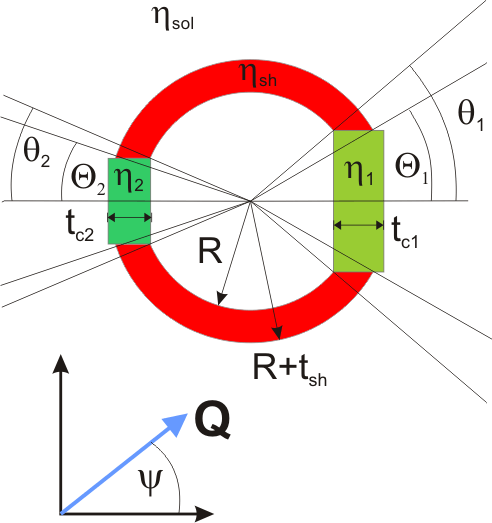
\includegraphics[width=0.492\textwidth]{vesicle_capped_poles_aligned.png}
\end{center}
\caption{Sketch of a vesicle with horizontally aligned flat
capped ends perpendicular to the incoming neutron beam}
\label{fig:Sketch_vesicle_capped_poles_aligned}
\end{figure}
The shape of this form factor consist of spherical vesicle containing to flat domains.
The flat thought to be aligned in a horizontal magnetic field perpendicular to the incoming
neutron beam. The size of the domains are characterized by the angles $\theta_1$ and
$theta_2$. The thicknesses $t_{c1}$ and $t_{c2}$ can be different than the thickness $t_{sh}$
of the spherical part of the vesicles. The same hold for the scattering length densities
$\eta_{c1}$, $\eta_{c2}$ and $\eta_{sh}$. The form factor $F_\text{cv}(Q)$ of this object can be
calculated by performing the Fourier transformation of the scattering length density in separate
steps. First one calculates the Fourier transformation of a sphere $F_\text{cSph}$
with flat capped ends on each side in cylinder coordinates.
\begin{subequations}
\begin{align}
F_\text{cSph}(Q,R,\psi,\theta_1,\theta_2,\Delta\eta) = \Delta\eta \!\!
\int_{-R\cos\theta_2}^{R\cos\theta_1} \!\!\!\!\! \mathrm{d}z \!\!\!
\int_0^{\sqrt{R^2-z^2}}\!\!\!\!\! \mathrm{d}\rho \;
\int_0^{2\pi} \mathrm{d}\phi \;\; e^{\imath \mathbf{Q}\cdot\mathbf{r}}
\, \rho
\label{eq:FcSphInt}
\end{align}
\begin{align}
\text{with} \quad
\mathbf{Q}=Q\left(
              \begin{array}{c}
                0 \\
                \sin\psi \\
                \cos\psi
              \end{array}
            \right)
\quad \text{and} \quad
\mathbf{r}= \left(
              \begin{array}{c}
                \rho \cos\phi \\
                \rho \sin\phi \\
                z
              \end{array}
            \right)
\end{align}
\end{subequations}
The form factor of vesicle $F_\text{cv}(Q)$ with a layer thickness of $t_\text{sh}$ can than
be calculated by
\begin{subequations}
\begin{align}
F_\text{cv}(Q,R,t_\text{sh},\theta_1,\theta_2,\Delta\eta_\text{sh}) =
    & + F_\text{cSph}(Q,R+t_\text{sh},\Theta_1,\Theta_2,\Delta\eta_\text{sh}) \nonumber \\
    & - F_\text{cSph}(Q,R,            \theta_1,\theta_2,\Delta\eta_\text{sh})
\end{align}
with
\begin{align}
\Theta_1 &= \arcsin\left(\frac{R_{c1}}{R+t_\text{sh}} \right), \quad R_{c1} = R \sin\left(\theta_1\right),\\
\Theta_2 &= \arcsin\left(\frac{R_{c2}}{R+t_\text{sh}} \right), \quad R_{c2} = R \sin\left(\theta_2\right).
\end{align}
\end{subequations}
As the flat capped ends are allowed to have independent thicknesses $t_\text{c1}$, $t_\text{c2}$ and
scattering length densities $\eta_\text{1}$, $\eta_\text{2}$ the scattering amplitude contribution of the
flat capped ends, which have the shape of a disc, need to be corrected. Their contribution can be calculated by
\newlength\breite
\settowidth\breite{$\displaystyle {}+{}$}
\begin{multline}
\begin{split}
F_\text{c}(Q,R,\theta_1,\theta_2,\dots) =
& \hspace{\breite} F_\text{c1}(Q,R,\theta_1,\Delta\eta_\text{c1}) - F_\text{d1}(Q,R,t_\text{d1},\Delta\eta_\text{sh}) \\
& +                F_\text{c2}(Q,R,\theta_2,\Delta\eta_\text{c2}) - F_\text{d2}(Q,R,t_\text{d2},\Delta\eta_\text{sh})
\end{split} \\[2mm]
\begin{split}
= & \hspace{\breite} \Delta\eta_\text{c1} \!\!\!
\int_{l_\text{c1}}^{l_\text{c1}+t_\text{c1}} \!\!\!\!\!
\mathrm{d}z\int_0^{R_\text{c1}} \!\!  \mathrm{d}\rho \int_0^{2\pi}\!\! \mathrm{d}\phi \; e^{\imath \mathbf{Q}\cdot\mathbf{r}}
\, \rho
- \Delta\eta_\text{sh} \!\!\!
\int_{l_\text{c1}}^{l_\text{c1}+t_\text{d1}} \!\!\!\!\!
\mathrm{d}z\int_0^{R_\text{c1}} \!\! \mathrm{d}\rho \int_0^{2\pi}\!\! \mathrm{d}\phi \; e^{\imath \mathbf{Q}\cdot\mathbf{r}}
\, \rho  \\
& + \Delta\eta_\text{c2} \!\!\!\!\!\!\!
\int_{-(l_\text{c2}+t_\text{c2})}^{-l_\text{c2}} \!\!\!\!\!\!\!\!
\mathrm{d}z\int_0^{R_\text{c2}} \!\! \mathrm{d}\rho \int_0^{2\pi}\!\!\mathrm{d}\phi \; e^{\imath \mathbf{Q}\cdot\mathbf{r}}
\, \rho
- \Delta\eta_\text{sh} \!\!\!\!\!\!\!
\int_{-(l_\text{c2}+t_\text{d2})}^{-l_\text{c2}} \!\!\!\!\!\!\!\!
\mathrm{d}z\int_0^{R_\text{c2}} \!\! \mathrm{d}\rho  \int_0^{2\pi}\!\!\mathrm{d}\phi \; e^{\imath \mathbf{Q}\cdot\mathbf{r}}
\, \rho \label{eq:Fc}
\end{split}
\end{multline}
with
\begin{subequations}
\begin{align}
\Delta\eta_\text{sh} &= \eta_\text{sh}-\eta_\text{sol}, \, \Delta\eta_\text{c1} = \eta_1-\eta_\text{sol} , \,
\Delta\eta_\text{c2} = \eta_2-\eta_\text{sol} \\
l_\text{c1} &= R\cos{\theta_1}, \, l_\text{c2} = R\cos{\theta_2} \\
R_\text{c1} &= R\sin{\theta_1}, \, R_\text{c2} = R\sin{\theta_2} \\
t_\text{d1} &= \sqrt{\left(R+t_\text{sh}\right)^2-R_\text{c1}^2}-\sqrt{R^2-R_\text{c1}^2} \\
t_\text{d2} &= \sqrt{\left(R+t_\text{sh}\right)^2-R_\text{c2}^2}-\sqrt{R^2-R_\text{c2}^2} \\
\end{align}
\end{subequations}
The solution of the integrals in eq.\ \ref{eq:FcSphInt} and \ref{eq:Fc} are
\begin{subequations}
\begin{multline}
F_\text{cSph}(Q,R,\psi,\theta_1,\theta_2,\Delta\eta) = \Delta\eta \!\!
\int_{-R\cos\theta_2}^{R\cos\theta_1} \!\!\!\!\! \mathrm{d}z \!\!\!
\int_0^{\sqrt{R^2-z^2}}\!\!\!\!\! \mathrm{d}\rho \;
\int_0^{2\pi} \mathrm{d}\phi \;\; e^{\imath \mathbf{Q}\cdot\mathbf{r}}
\, \rho  \\
 \Delta\eta \!\!
\int_{-R\cos\theta_2}^{R\cos\theta_1} \!\!\!\!\! \mathrm{d}z\;\;
\exp\left(\imath Q z \cos\psi\right)  2\pi \left(R^2 - z^2\right)
\frac{J_1\left(Q \sqrt{R^2 - z^2} \sin\psi\right)}{Q \sqrt{R^2 - z^2} \sin\psi}
\label{eq:FcSphPsi}
\end{multline}
and
\begin{multline}
F_\textrm{c$_i$,d$_i$}(Q,R_\textrm{c$_i$,d$_i$},\psi,\Delta\eta)   =
\Delta\eta \int_{a}^{b}\!\! \mathrm{d}z
           \int_0^{R_\textrm{c$_i$}}\!\! \mathrm{d}\rho
           \int_0^{2\pi}\!\! \mathrm{d}\phi \;\; e^{\imath \mathbf{Q}\cdot\mathbf{r}}
\, \rho \\
 = 4 \pi R \frac{\imath \left(\exp\left(\imath a Q \cos\psi\right)-\exp\left(\imath b Q \cos\psi\right)\right)
 J_1\left(Q R \sin\psi\right)}{\sin\left(2\psi\right) Q^2}
\end{multline}
\end{subequations}
whereby $\mathrm{J}_1$ the regular cylindrical Bessel function of first order.
The overall scattering intensity $I_{\textrm{alignedVes}}(Q,\psi,\dots)$ is finally given by
\begin{align}
I_{\textrm{alignedVes}}(Q,\psi,\dots) =
\abs{
 F_\text{cv}(Q,R,\psi,t_\text{sh},\theta_1,\theta_2,\Delta\eta_\text{sh})
+F_\text{c}(Q,R,\psi,\theta_1,\theta_2,\dots)}^2
\end{align}
\vspace{5mm}
\begin{sloppypar}
\noindent \underline{Input Parameters for the models of \texttt{MagneticFieldAlignedVesicle}:}
\end{sloppypar}
\begin{description}
\item[\texttt{Rsh}] radius of spherical vesicle shell
\item[\texttt{theta1}] angle to describe size of first capped side
\item[\texttt{theta2}] angle to describe size of second capped side
\item[\texttt{t\_sh}] thickness of spherical vesicle shell
\item[\texttt{t\_c1}] thickness of first flat capped side
\item[\texttt{t\_c2}] thickness of second flat capped side
\item[\texttt{eta\_sh}] scattering length density of spherical vesicle shell
\item[\texttt{eta\_1}] scattering length density of first capped side
\item[\texttt{eta\_2}] scattering length density of second capped side
\item[\texttt{eta\_sol}] scattering length density of solvent
\end{description}

\noindent\underline{Note:}
\begin{itemize}
\item[~] None
\end{itemize}

\begin{figure}[htb]
\begin{center}
%\includegraphics[width=0.768\textwidth]{sphere_P.png}
\end{center}
%\caption{Scattering intensity of spheres with radii $R=10$nm and $R=20$nm.
%The scattering length density contrast is set to 1.} \label{fig:I_sphere}
\end{figure}
